\chapter{🏞️ Allometry: How organismal characteristics vary with size}

One area in which Organismal Biologists use these ideas is in the study of \href{https://en.wikipedia.org/wiki/Allometry}{allometry}.
Allometry is the study of how organismal traits vary systematically with body length or similar metrics of size.
Allometric relationships have been found or hypothesized for many traits, including mass, morphology of limbs and other structures, locomotion and other behaviors, and physiological characteristics such as respiration and nutrient uptake.

A well-known example of an allometric relationshop is \href{https://en.wikipedia.org/wiki/Kleiber's\_law}{Kleiber's law}, which posits that the basal metabolic rate of animals varies approximately as the animal's mass raised to the $\frac{3}{4}$ power:

\begin{figure}[!htbp]
\centering
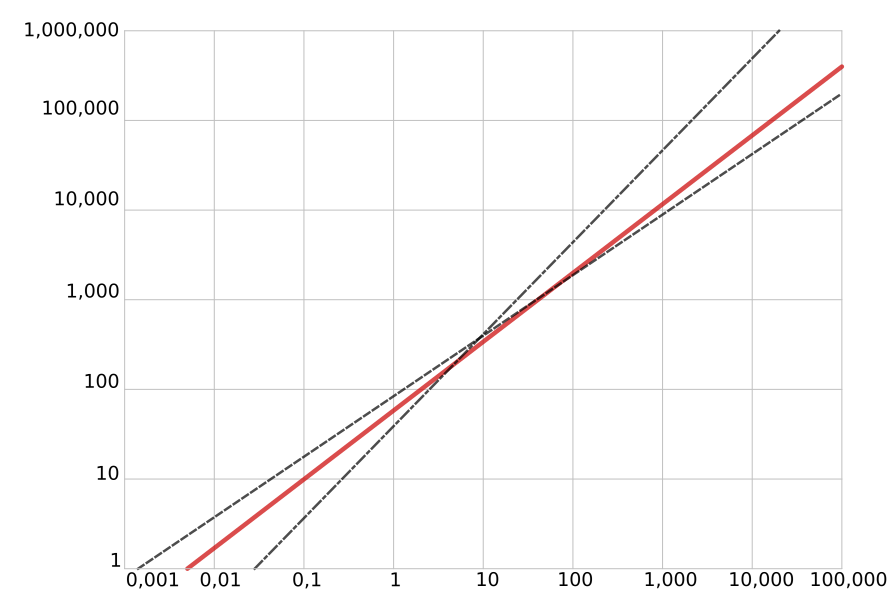
\includegraphics[width=0.625\linewidth]{files/f51f7dfbc9ea77c954642c24a07009ce.pdf}
\caption[]{A plot of Kleiber's law, relating the metabolic rates of organisms to their sizes across a large range of sizes. See the Wikipedia article on \href{https://en.wikipedia.org/wiki/Kleiber's\_law}{Kleiber's law} for details.}
\label{Kleiber}
\end{figure}

Allometric relationships within taxonomic groups are usually determined by statistical analysis of observations across a range of organism sizes within the group.
These observations are most commonly plotted on log-log plots, and statistically analyzed to detect trends.
A line on a log-log plot represents a power law relationship, which can be expressed mathematically as
\begin{equation}
\label{K1}
trait = c~size^p,
\end{equation}
where $c$ is a constant, and $p$ is an exponent indicating the type of allometry.
Taking the log of both sides of [\#K1] gives
\begin{equation}
\label{K2}
\log{trait} = \log{c} + p \times \log{ size}.
\end{equation}
[\#K2] shows why power law allometries appear at straight lines on log-log plots.

For example, in Figure~\ref{Kleiber}, the trait is \href{https://en.wikipedia.org/wiki/Basal\_metabolic\_rate}{Basal Metabolic Rate} in watts, $BMR$, the size metric is mass, $M$, the constant $c = 70$, and the hypothesized exponent is $p=\frac{3}{4}$, \textit{i.e.},
\begin{equation}
BMR = 70~ M^\frac{3}{4}
\end{equation}
It is useful to distinguish two types of allometry, \textit{isometric scaling} and \textit{allometric scaling}.

\section{Isometric scaling}

Isometric scaling is also known as \textit{geometrical similarity}.
In isometric scaling, all linear proportions are held constant as overall size increases or decreases.
The spherical egg model in \href{/example}{the previous notebook} is an example of isometric scaling.
In general, a series of isometrically scaled objects follow the so-called \href{https://en.wikipedia.org/wiki/Square-cube\_law}{square-cube law}, stating that surface area is proportional to the length squared, and volume is proportional to length cubed.

\section{Allometric scaling}

In allometric scaling, different organismal traits scale differently with metrics of size.
For example, larger animals often have more robust bones than would be predicted by isometric scaling from smaller animals.
In a given organism, different traits may reflect either direct or indirect effects of isometric and allometric scaling.

For example, if a set of animals scaled isometrically, their weight might be expected to increase in proportion to the cube of their length.
However, following the \href{https://en.wikipedia.org/wiki/Square-cube\_law}{square-cube law}, the cross-sectional area of their bones would increase only in proportion to the square of their length.
This is likely to result in much higher loading and risk of breakage in larger animals.

In this case, some traits of these animals might deviate from isometric scaling, and instead follow an allometric scaling.
For example, bones might increase in thickness faster than isometrically, or mass might increase slower than isometrically.
Either form of allometric scaling would tend to equalize the loading on bones, relative to isometric scaling.